%%%%%%%%%%%%%%%%%%%%%%%%%%%%%%%%%%%%%%%%%%%%%%%%%%%%%
\chapter{Introduction} \label{chap:intro}
\graphicspath{{images/intro/}}

\gls{hri} what it is and what it matters and why it is challenging

Robots will inhabit human spaces and need to interact with them in decent ways

Robot behaviour unlikely to be programmable and static

This works explores how robots could interact with humans to learn from them to interact with other humans

%%%%%%%%%%%%%%%%%%%%%%%%%%%%%%%%%%%%%%%%%%%%%%%%%%%%%
\section{Scope}\label{sec:intro-scope}

Enabling a robot to interact socially with humans is complex task. The robot needs to interpret a large sensory space, relying on images camera, motor joints or high level concepts defining the state of the interaction. Then based on the interpretation of this inputs and rules defining expected behaviour or limiting the behaviour, the robot needs to select an action or a plan it will execute to fit the goal it has been assigned. The following sections will aim to refine the scope of the research conducted in this thesis.

\subsection{Frame}

The focus of the research conducted here is finding a way for robots to interact safely and efficiently with humans. It has been argued by many \citep{dautenhahn2004robots,billard2008robot} that an efficient robot interacting with human would not be preprogrammed beforehand and execute a one-size-fits-all policy suited to every possible interaction partners. Robots needs to be able to learn an interactive behaviour, improving their skills as they interact and personalising their policy to the preferences of their users. The aim of this thesis is finding a interaction framework allowing humans to teach robot how to interact with other humans.  

Throughout this thesis we make the assumption that, while an engineer designing a robot behaviour might not know how the robot should behave, an expert possess this knowledge and should be able to transfer it to the robot. This human teacher's expertise is not related to theoretical knowledge in \gls{ml}, robotics or other scientific fields. It just denotes that this person possess knowledge unknown by the engineer design the robot. This could take the form of the steps of a therapy a robot should deliver to the child (known by a therapist) or more simply a senior's preferences and desires concerning a robot companion.

This thesis aims to provide a convenient and efficient way for this domain expert to inculcate this knowledge in the robot.


\subsection{Environment} 

Robots considered in this thesis evolve in human-centred environment and are expected to provide some support to the surrounding humans and achieve a specific goal assigned to them. Interactions with humans are by essence social, and robots needs to take into these social norms when interacting in human environments.

???

\subsection{Type of interaction}

The typical interaction considered in this thesis is a triadic interaction between a human the user of the robot, the robot and an application target, potentially another human (as shown in Figure \ref{fig:intro_setup}). In this type of interaction, the user has an aim for robot, a task they would like the robot to complete. And through the teaching interaction, they can supervise the robot, demonstrating it what it should do and teaching it an efficient action policy in the application interaction with the target.

The application target could be another human (such as a child receiving teaching support from the robot) or just parts of the environment if the robot has to complete a manipulation of navigation task (such as picking up a book in the library).

\begin{figure}[ht]
	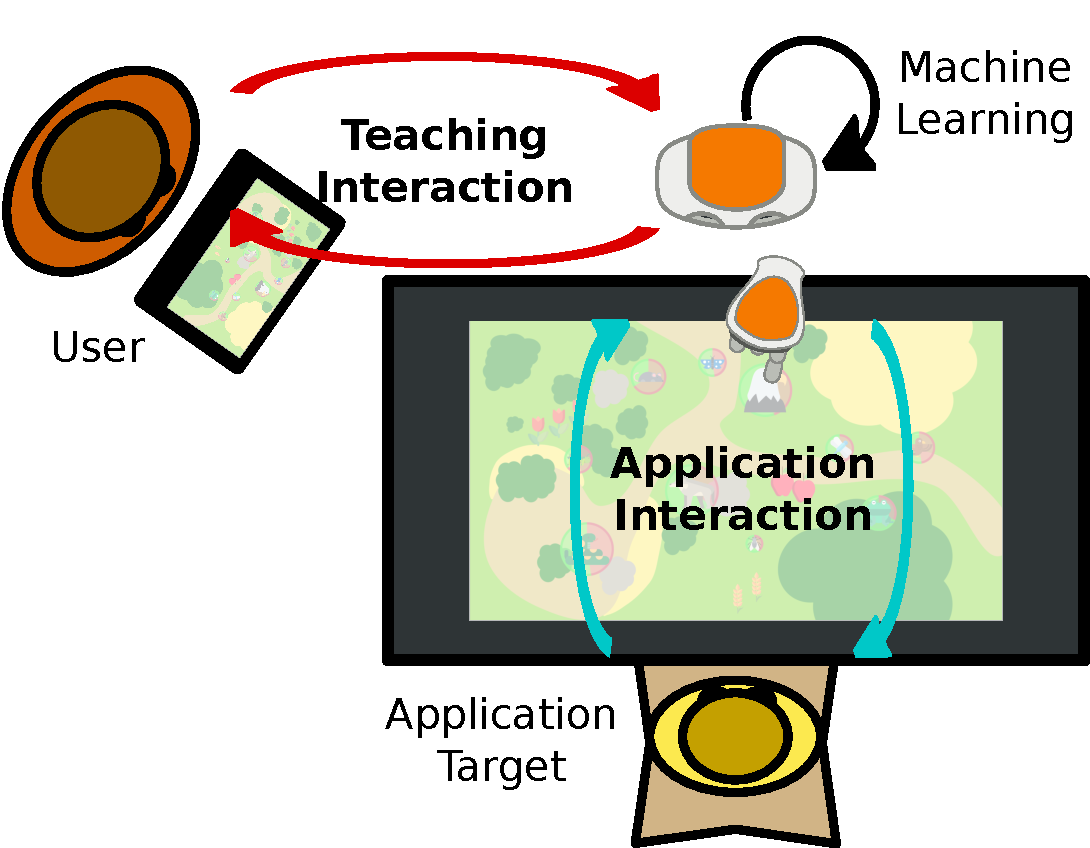
\includegraphics[width=.7\linewidth]{setup.pdf}
	\centering
	\caption{The typical interaction used in this research: a robot interacts with a target in an application interaction and learns from a domain expert through a teaching interaction.}
	\label{fig:intro_setup}
\end{figure}

\subsection{Algorithms}

The aim of this thesis being exploring how humans could teach robots to interact in  human-centred environment, the robot needs to possess a learning algorithm allowing it to improve its action policy. Two main categories of learning algorithms have been used in this research: \gls{sl} and \gls{rl}.

\gls{sl} aims to learn a mapping between inputs and outputs to automatically reproduce a desired behaviour. It uses a dataset of labelled example and optimise an algorithm such as its prediction error of the output for each input is minimised \citep{russell2016artificial}. Typical example used in this study are \gls{ann} and nearest neighbours methods. \gls{ann} models loosely the way brains and neurons work by having a group of `neurons' connected between each other by synapses. Each neuron updates its according value according to connections with other neurons including weights and non-linearity. The general approach have a set of input nodes, a set of output nodes and hidden nodes, and the network learns by changing the value of the weights to reproduce the desired values on the output nodes. Nearest neighbours methods compare the distance in the feature space between a point to classify to the different instances stored in a dataset and select the value of a majority of nearest neighbours in this space.

Unlike \gls{sl} which aims at reproducing a known behaviours, \gls{rl} aims at providing an agent with the capacity to discover the world it interact in and learn from this interaction with the world \citep{sutton1998reinforcement}. The agent has access to a description of the state and actions it can do, and depending of the action selected, the state will change and the agent will receive a reward. The goal of the agent is to find an optimal policy maximising a notion of cumulated reward.

Due to the relevance of both fields to this thesis research topics: enabling humans to teach robots to interact, algorithm from both categories have been used. The first study presented in Chapter \ref{chap:woz} uses a feed forward neural network learning to reproduce a teacher policy. The second study in Chapter \ref{chap:control} used \acrlong{rl} combining human and environmental rewards. The aim of this algorithm is to use the human guidance and rewards to learn an efficient interaction policy. And the last study presented in Chapter \ref{chap:tutoring} uses instance based algorithm adapted from Nearest Neighbours to enable quick and efficient learning. More details about each algorithms and their related work can be found in the associated chapters.

%%%%%%%%%%%%%%%%%%%%%%%%%%%%%%%%%%%%%%%%%%%%%%%%%%%%%
\section{The Thesis}\label{sec:intro-thesis}
The main thesis that this document seeks to put forward is as below.
\begin{quote}
	A robot can learn how to interact meaningfully with humans by receiving supervision from a human teacher in control of the robot's behaviour, this supervision will lead to an efficient, safe and low human-workload teaching and autonomous behaviour.	
\end{quote}
%One sentence to describe the take home/conclusion

Additional research questions have been explored during the progress of this
work and are introduced here.

\begin{itemize}
    \item \textbf{What kind of interaction could allow a human to teach a robot to interact with other humans while ensuring an appropriate and adaptive interaction policy and a low workload on the human teacher?}
    
    	Justification for \gls{sparc} 
    \item \textbf{Does adding a learning component to a supervised robot can reduce the human-workload of the supervisor?}
    
        \gls{woz} is an approach widely used in \gls{hri} \citep{riek2012wizard}, whereby a human teleoperates a robot to have it interact with other humans. However, this method applies a high workload on the operator and is not scalable. Using \gls{ml} to learn from this operator online might decrease the operator's workload without decreasing the quality of the robot behaviour.
    
    \item \textbf{How control of a teacher over the robot's action impacts the robot's learning?} 
    
	    In the context of \gls{iml}, a human can provide inputs to an agent to speed up the learning. Other \gls{iml} \citep{thomaz2008teachable,knox2009interactively} focus on feedback from the human with limited or no control over the agent's actions. However increase the control should speed up the learning and reduce the number of errors made by the robot.

    \item \textbf{After receiving supervision from a human, could a robot behave autonomously in a social context?}

	 	\gls{sparc} has been designed to allow non-experts in \gls{ml} to teach agents how to interact while interacting. Human-robot interactions provide a perfect test for this approach: using a human to teach a robot how to behave in this complex and non-deterministic environment.
	 
\end{itemize}

%%%%%%%%%%%%%%%%%%%%%%%%%%%%%%%%%%%%%%%%%%%%%%%%%%%%%
\section{Approach and Experimentation}\label{sec:intro-exps}

introduction of structure, and especially why it is that way

why literature review, why and conclusion

how the results have been used to design a new interaction framework to teach robots to interact with humans

how it has been tested and why that order

%%%%%%%%%%%%%%%%%%%%%%%%%%%%%%%%%%%%%%%%%%%%%%%%%%%%%
\section{Key Concepts and terminology}\label{sec:intro-concepts}

Not sure if worth including

Throughout this thesis, the terms `wizard', `supervisor', `user', `expert' and `teacher' have been used interchangeably to represent the people in control of a robot's action and teaching that robot an action policy.

agent and robot

\begin{itemize}
	\item \textbf{Appropriateness}:
	\item \textbf{Adaptivity}
	\item \textbf{Autonomy}
	\item \textbf{Supervised Autonomy}
	\item \textbf{Learning}
	\item \textbf{Teacher, wizard, user, expert and supervisor}
	\item \textbf{Robot and agent}
\end{itemize}

%%%%%%%%%%%%%%%%%%%%%%%%%%%%%%%%%%%%%%%%%%%%%%%%%%%%%
\section{Challenges}

Complexity of interactions with humans: complex world, safety, workload and so on

%%%%%%%%%%%%%%%%%%%%%%%%%%%%%%%%%%%%%%%%%%%%%%%%%%%%%
\section{Contributions}\label{sec:intro-contr}

\subsection{Scientific contribution}
\begin{itemize}
	\item Design of a new interaction framework for teaching agents in a safe way.
	\item Evaluation in three studies.
	\item Demonstration of the importance of control over the robot's action when teaching a robot to interact.
	\item Design of a lightweight algorithm to quickly learn from demonstration in complex environments.
	\item Application of \gls{iml} to safely teach robots social autonomy from in situ human supervision. 
	\item Software development for two projects: \acrshort{dream} (European FP7 project: 611391) and Human-Robot Interaction Strategies for Rehabilitation based on Socially Assistive Robotics (Royal Academy of Engineering: IAPP\textbackslash1516\textbackslash137).
\end{itemize}

\subsection{Technical contribution}

%%%%%%%%%%%%%%%%%%%%%%%%%%%%%%%%%%%%%%%%%%%%%%%%%%%%%
\section{Structure}\label{sec:intro-struct}
The structure of this thesis is outlined below to provide an overview of the content and context for each chapter. A summary of key experimental findings are included at the start of each relevant chapter for ease of reference. 

\begin{itemize}
	\item This chapter provided an introduction to the general field of this research (robots learning to interact with humans), the research questions including the central \textit{thesis}, scope, and contributions of the work presented in later chapters.  

	\item Chapter~\ref{chap:background} provides a description of the different fields of \gls{hri} and draws three requirements for robot's controllers interacting with humans. In a second part, it analyses the current controllers for robots in \gls{hri} identifying that no current controller fits these requirements. Finally, it proposes to apply \gls{iml} to \gls{hri} to validate the requirements, which is the goal of this thesis.
	
	\item Chapter~\ref{chap:sparc} proposes a new interaction framework, \gls{sparc}, aiming to provide a way to apply \gls{iml} to \gls{hri} while validating the three requirements proposed in Chapter \ref{chap:background}. Additionally, this chapter presents the expectations of \gls{sparc}.
	
	\item Chapter~\ref{chap:woz} presents results from a first study evaluating if the principles of \gls{sparc} would allow to reduce the workload on a supervisor compared to \gls{woz}. Results support the hypotheses, validating some of the motivation of \gls{sparc} (a learning robot would reduce the workload on a supervisor).
	
	\item Chapter~\ref{chap:control} presents results from a second study comparing \gls{sparc} to \gls{irl}, another interaction framework from \gls{iml}. The main difference between the two approaches is the amount of control the teacher has. With \gls{sparc}, the teacher can correct any action executed by the robot, and results support that this control improves the efficiency of the learning (performance, time and inputs required to teach and risks taken during the teaching phase).
	
	\item Chapter~\ref{chap:tutoring} presents a study where \gls{sparc} has been applied to a real world \gls{hri}, child tutoring. And results demonstrate that while not impacting the learning gain of the session, an autonomous robot having learned using \gls{sparc} elicit similar children behaviour than a supervised robot, unlike a passive robot. This results support \gls{sparc} as a teaching method allowing to transfer a social and technical action policy from human expert to a robot in a safe way.
	
	\item Chapter~\ref{chap:discussion} presents a discussion from the main findings from the previous chapters and presents limitations and future directions of research for \gls{sparc}.
	
	\item Chapter~\ref{chap:conclusion} concludes the thesis and presents a summary of the main contributions.
	
\end{itemize}
